%% Overleaf			
%% Software Manual and Technical Document Template	
%% 									
%% This provides an example of a software manual created in Overleaf.

\documentclass{../ol-softwaremanual}

% Packages used in this example
\usepackage{graphicx}  % for including images
\usepackage{microtype} % for typographical enhancements
\usepackage{minted}    % for code listings
\usepackage{amsmath}   % for equations and mathematics
\setminted{style=friendly,fontsize=\small}
\renewcommand{\listoflistingscaption}{List of Code Listings}
\usepackage{hyperref}  % for hyperlinks
\usepackage[a4paper,top=4.2cm,bottom=4.2cm,left=3.5cm,right=3.5cm]{geometry} % for setting page size and margins

\usepackage[english, greek]{babel}

\usepackage{subfig}


% Custom macros used in this example document
\newcommand{\doclink}[2]{\href{#1}{#2}\footnote{\url{#1}}}
\newcommand{\cs}[1]{\texttt{\textbackslash #1}}

\begin{document}
	
	
	\begin{titlepage}
		
		
		% Frontmatter data; appears on title page
		\title{\en Risk Assessment \\}
		\version{0.2}
		\softwarelogo{
\includegraphics[scale=0.4]{../CarBazaar_logo.png}}
	\end{titlepage}
	
	
	\maketitle
	
	\newpage
	
	\center{\textbf{Μέλη Ομάδας}}
	
	\vspace{20pt}
	
	
	
	\begin{table}[htbp!]
		
		\begin{tabular}{llll}
			Μεμελετζόγλου Χαρίλαος & 1069364 & \en st1069364@ceid.upatras.gr & 4o Έτος   \\ 
			\\ Λέκκας Γεώργιος      &      1067430    &   \en st1067430@ceid.upatras.gr & 4o Έτος  \\
			\\ Γιαννουλάκης Ανδρέας        &   1067387       & \en st1067387@ceid.upatras.gr & 4o Έτος           \\
			\\ Κανελλόπουλος Ιωακείμ        &  1070914        &    \en st1070914@ceid.upatras.gr & 4o Έτος        \\ 
		\end{tabular}
	\end{table}
	
	\center{\textbf{Υπεύθυνοι Παρόντος Τεχνικού Κειμένου}}
	
	\vspace{20pt}
	
	\begin{table}[htbp!]
		\begin{tabular}{ll}
			Μεμελετζόγλου Χαρίλαος & \en Editor \\
			\\ Λέκκας Γεώργιος      &   \en  Contributor \\
			\\ Γιαννουλάκης Ανδρέας & \en Peer Reviewer \\
			\\ Καννελόπουλος Ιαωκείμ & \en Contributor \\ 
		\end{tabular}
	\end{table}

	\center{\textbf{Αλλαγές στην έκδοση \en v0.2 \gr}}
	\vspace{10pt}

	\begin{itemize}
		\item Προσθήκη του κινδύνου Νο. 7 (χαμηλός αριθμός χρηστών λόγω ύπαρξης παρόμοιων εφαρμογών)
		\item Προσθήκη του κινδύνου Νο. 8 (ψευδείς \en (fake) \gr αγγελίες)
	\end{itemize}

	
	
	\vspace{20pt}
	
	\center{\textbf{Εργαλεία που χρησιμοποιήθηκαν}}
	
	\vspace{20pt}
	\flushleft
	Χρησιμοποιήθηκε το \en \doclink{https://www.overleaf.com/}{Overleaf} \gr και το \en \doclink{https://www.texstudio.org/}{TexStudio} \gr για την συγγραφή του \LaTeX\ κώδικα. \break
	
	Για την δημιουργία και συμπλήρωση των φορμών κινδύνων, χρησιμοποιήθηκε το \en MS Word \gr και το \en OpenOffice\gr.
	
	
	
	
	\newpage 
	
	\center{\textbf{Πιθανοί Κίνδυνοι (Ανάλυση Κινδύνων κατά \en Boehm\gr)}}
	
	\flushleft
	
	\begin{figure}[htbp!]
		\includegraphics[scale=0.7]{img/wrong\_scheduling.png}
		\caption{Κίνδυνος Λάθος Χρονοπρογραμματισμού}
	\end{figure}
	
	\newpage
	
	
	
	\begin{figure}[htbp!]
		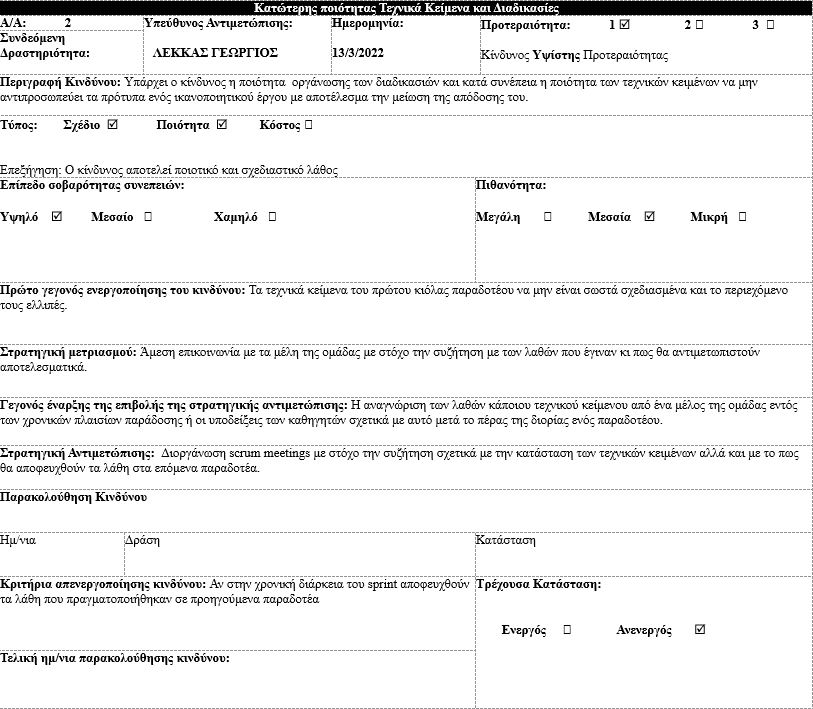
\includegraphics[scale=0.8]{img/bad quality.png}
		\caption{Κίνδυνος Ποιότητας}
	\end{figure}
	
	\newpage
	
	\begin{figure}[htbp!]
		\includegraphics[scale=0.7]{img/implementation\_changes.png}
		\caption{Κίνδυνος Διορθωτικών Κινήσεων κατά την Υλοποίηση}
	\end{figure}
	
	
	
	\newpage
	
	\begin{figure}[htbp!]
		\includegraphics[scale=0.7]{img/project\_cost.png}
		\caption{Κίνδυνος Εσφαλμένης Εκτίμησης Κόστους}
	\end{figure}
	
	\newpage
	
	\begin{figure}[htbp!]
		\includegraphics[scale=0.5]{img/Legal\_issues.png}
		\caption{Κίνδυνος Νομικών Ζητημάτων}
	\end{figure}
	
	
	\newpage
	
	\begin{figure}[htbp!]
		\includegraphics[scale=1]{img/Human\_Resources\_Issues.png}
		\caption{Kίνδυνος που αφορά το Ανθρώπινο Δυναμικό}
	\end{figure}

	\newpage

\begin{figure}[htbp!]
	\includegraphics[scale=0.8]{img/low\_user\_count.png}
	\caption{Kίνδυνος Χαμηλού Αριθμού Χρηστών}
\end{figure}
	
	\newpage
	\begin{figure}[htbp!]
		\includegraphics[scale=0.7]{img/fake\_listings.png}
		\caption{Kίνδυνος Ψευδών Αγγελιών}
	\end{figure}
	
	
	
\end{document}
